\section{Experimental Results}
I experimented this system on 7 people, including 6 famous actors from the movie Jurassic Park (1993) and
myself, with each of them given a student ID (e.g., U10516001). The training image set of the 6 actors is
from the tutorial [1] on pyimagesearch.
\newline

\begin{enumerate}
  \item U10516001 - Alan Grant (22 images)
  \item U10516002 - Claire Dearing (53 images)
  \item U10516003 - Ellie Sattler (31 images)
  \item U10516004 - Ian Malcolm (41 images)
  \item U10516005 - John Hammond (36 images)
  \item U10516006 - Owen Grady (35 images)
  \item U10516045 - Guan-Zhong Wang (5 images)
\end{enumerate}

It can distinguish between 7 different people, successfully automating a roll call, as shown in Figure 2.

\begin{figure}[h!]
  \centering
  \begin{subfigure}[b]{0.32\linewidth}
    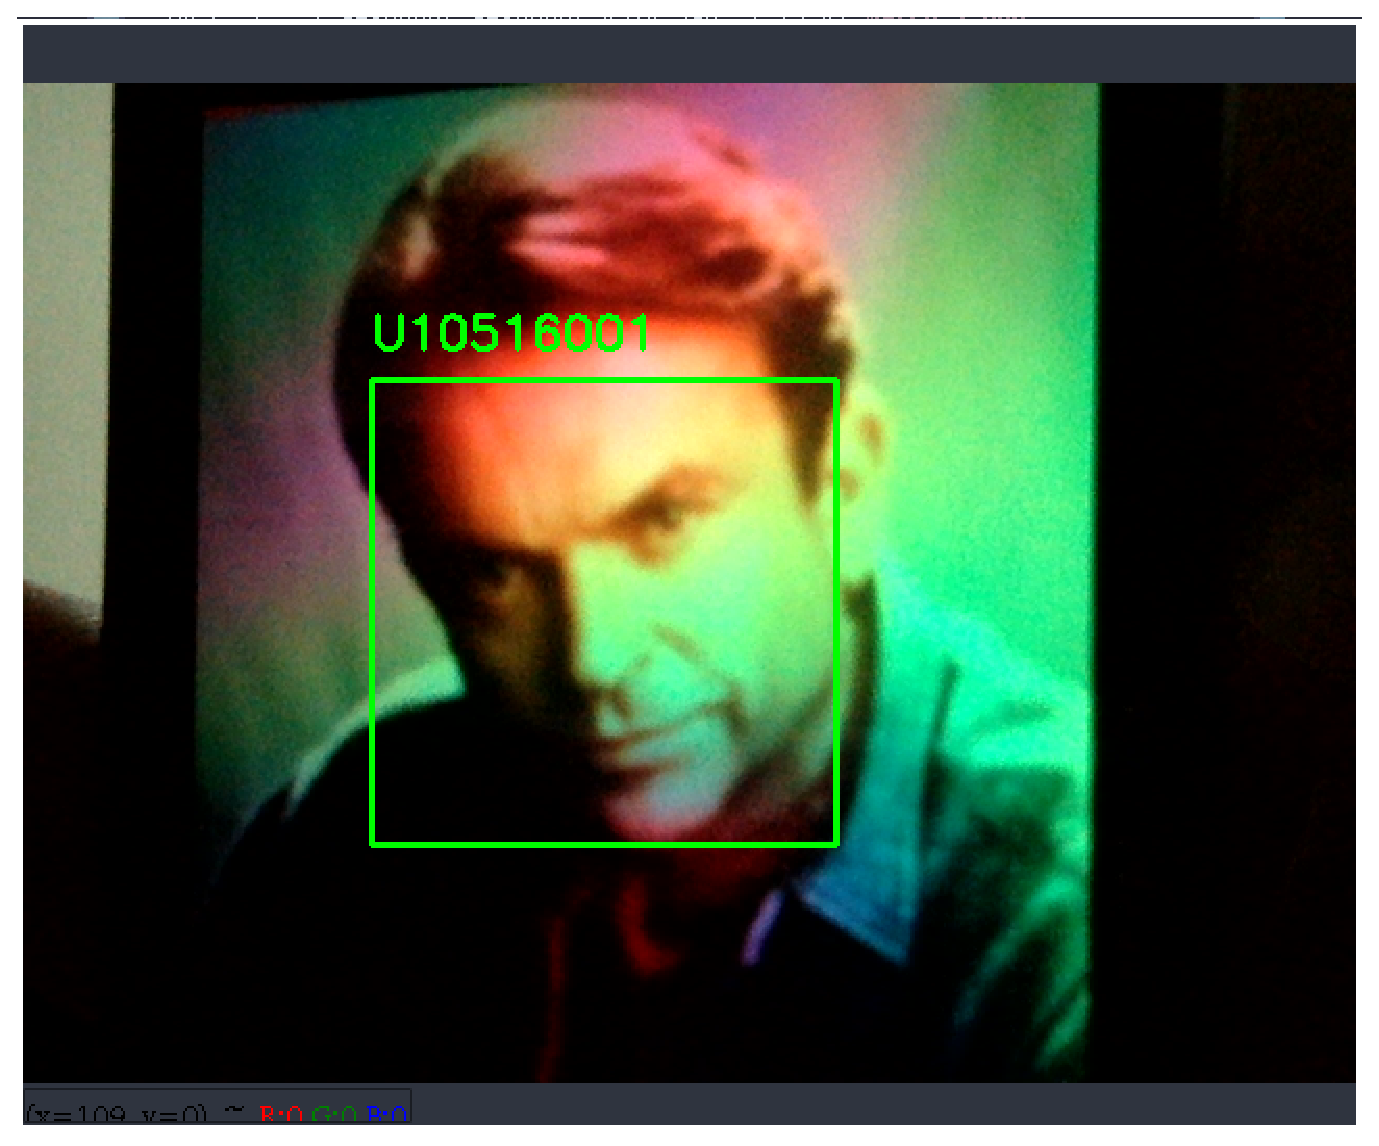
\includegraphics[width=\linewidth]{figures/exp01.eps}
    \caption{U10516001 Alan Grant.}
  \end{subfigure}
  \begin{subfigure}[b]{0.32\linewidth}
    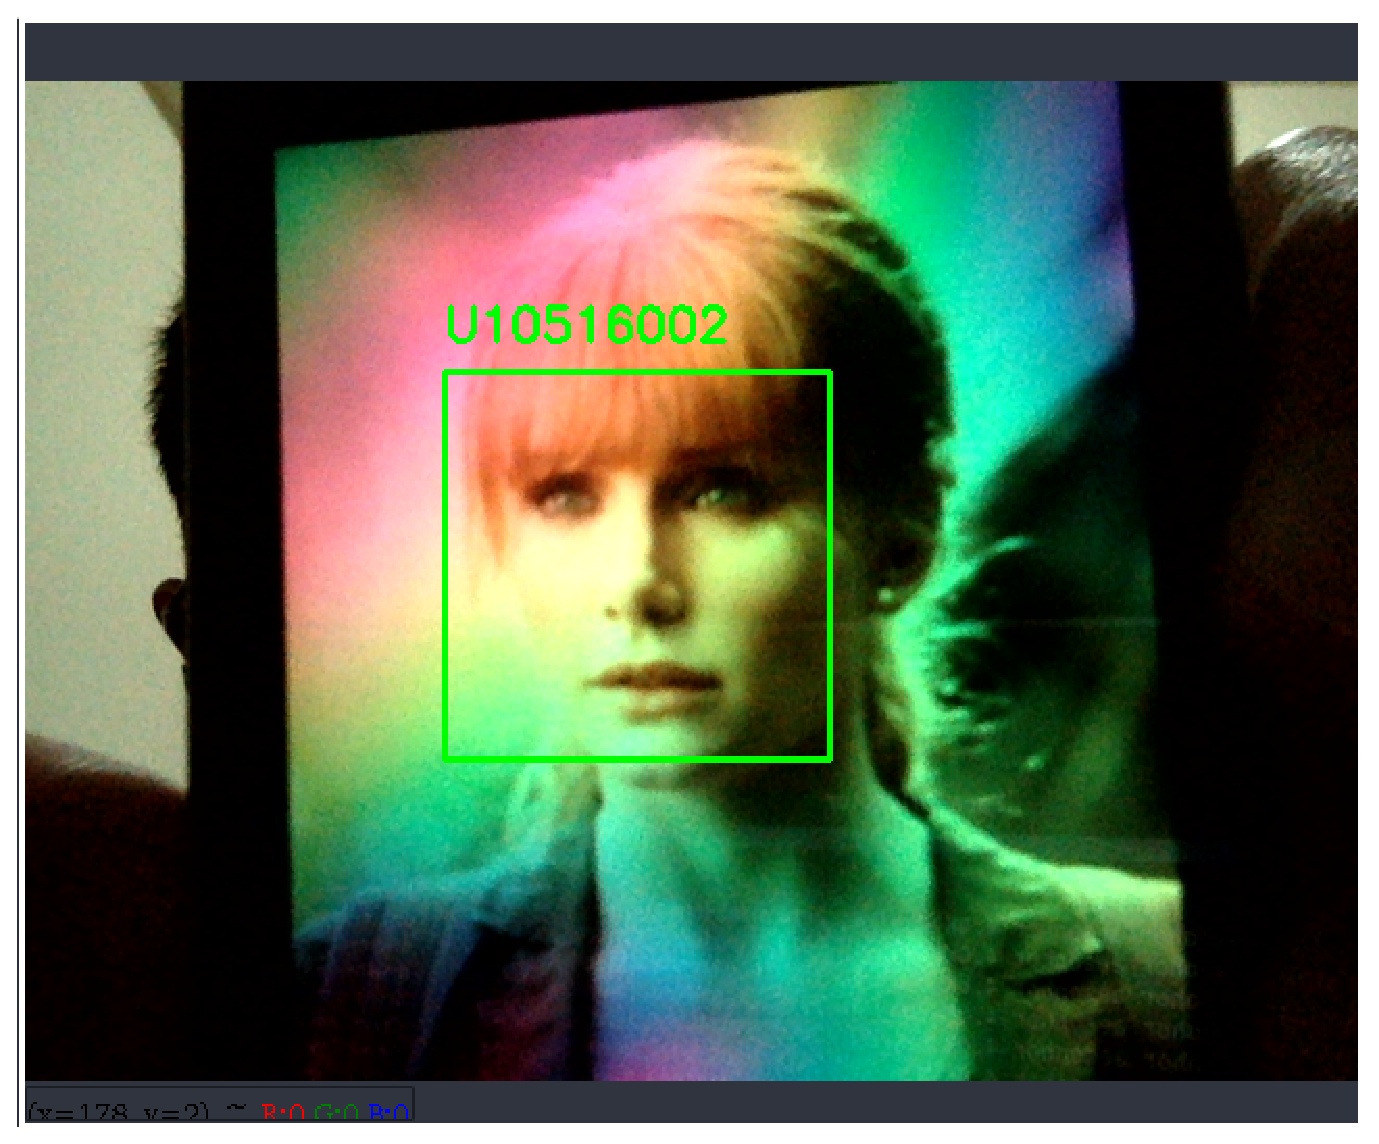
\includegraphics[width=\linewidth]{figures/exp02.eps}
    \caption{U10516002 Claire Dearing.}
  \end{subfigure}
  \begin{subfigure}[b]{0.32\linewidth}
    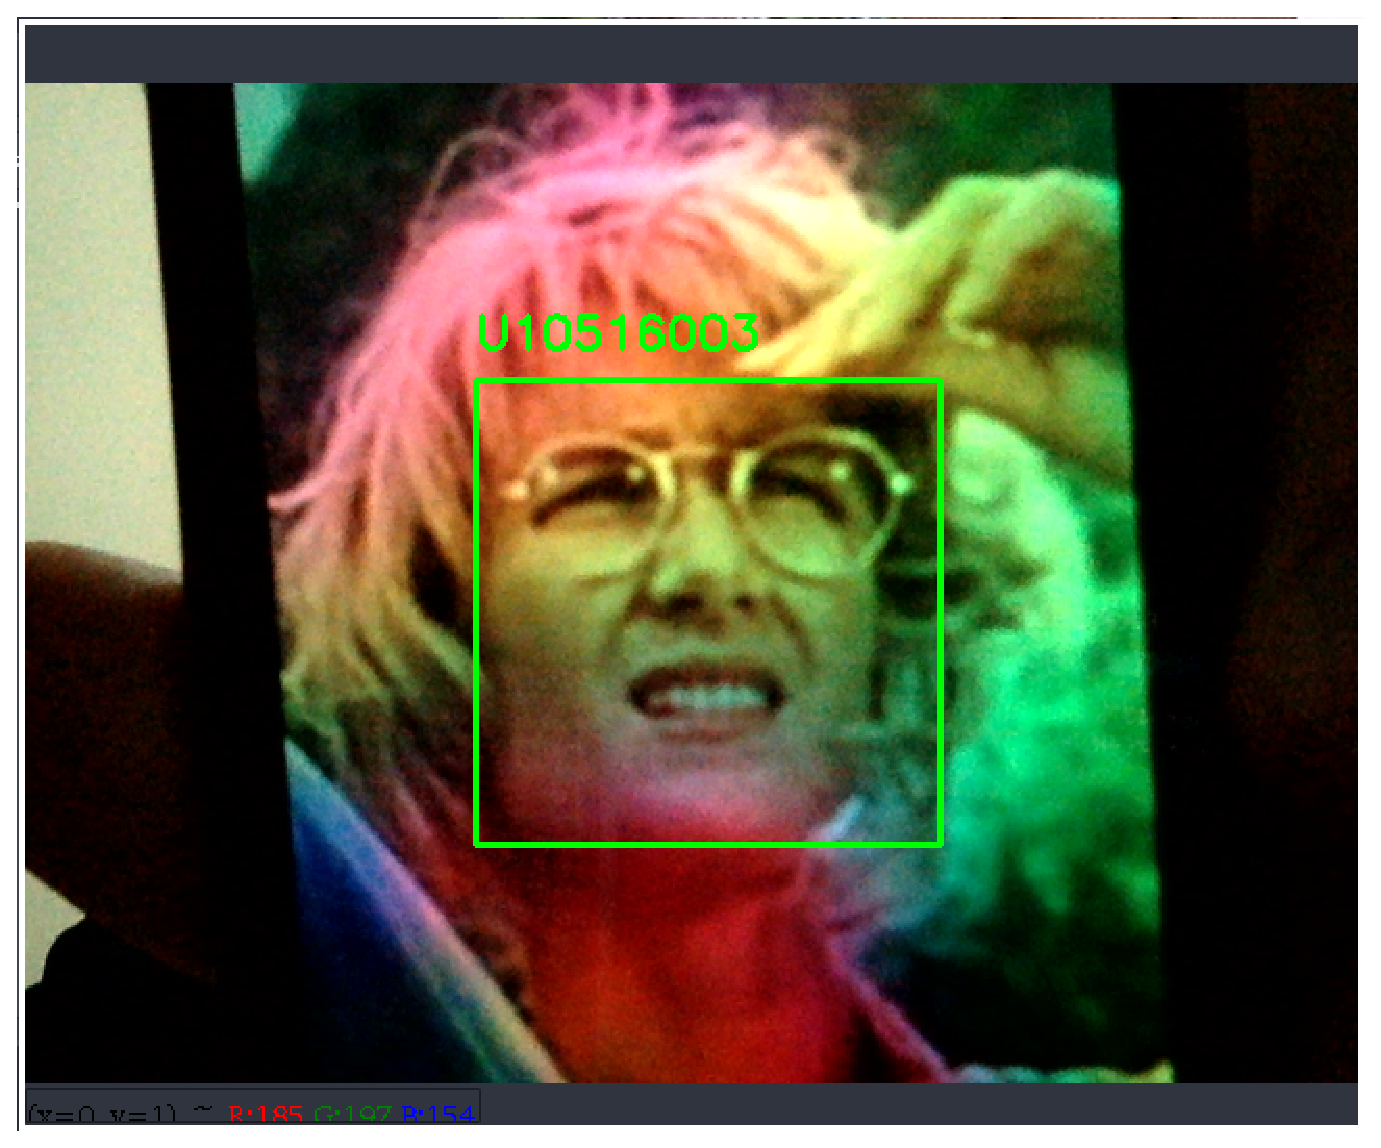
\includegraphics[width=\linewidth]{figures/exp03.eps}
    \caption{U10516003 Ellie Sattler.}
  \end{subfigure}
  \begin{subfigure}[b]{0.32\linewidth}
    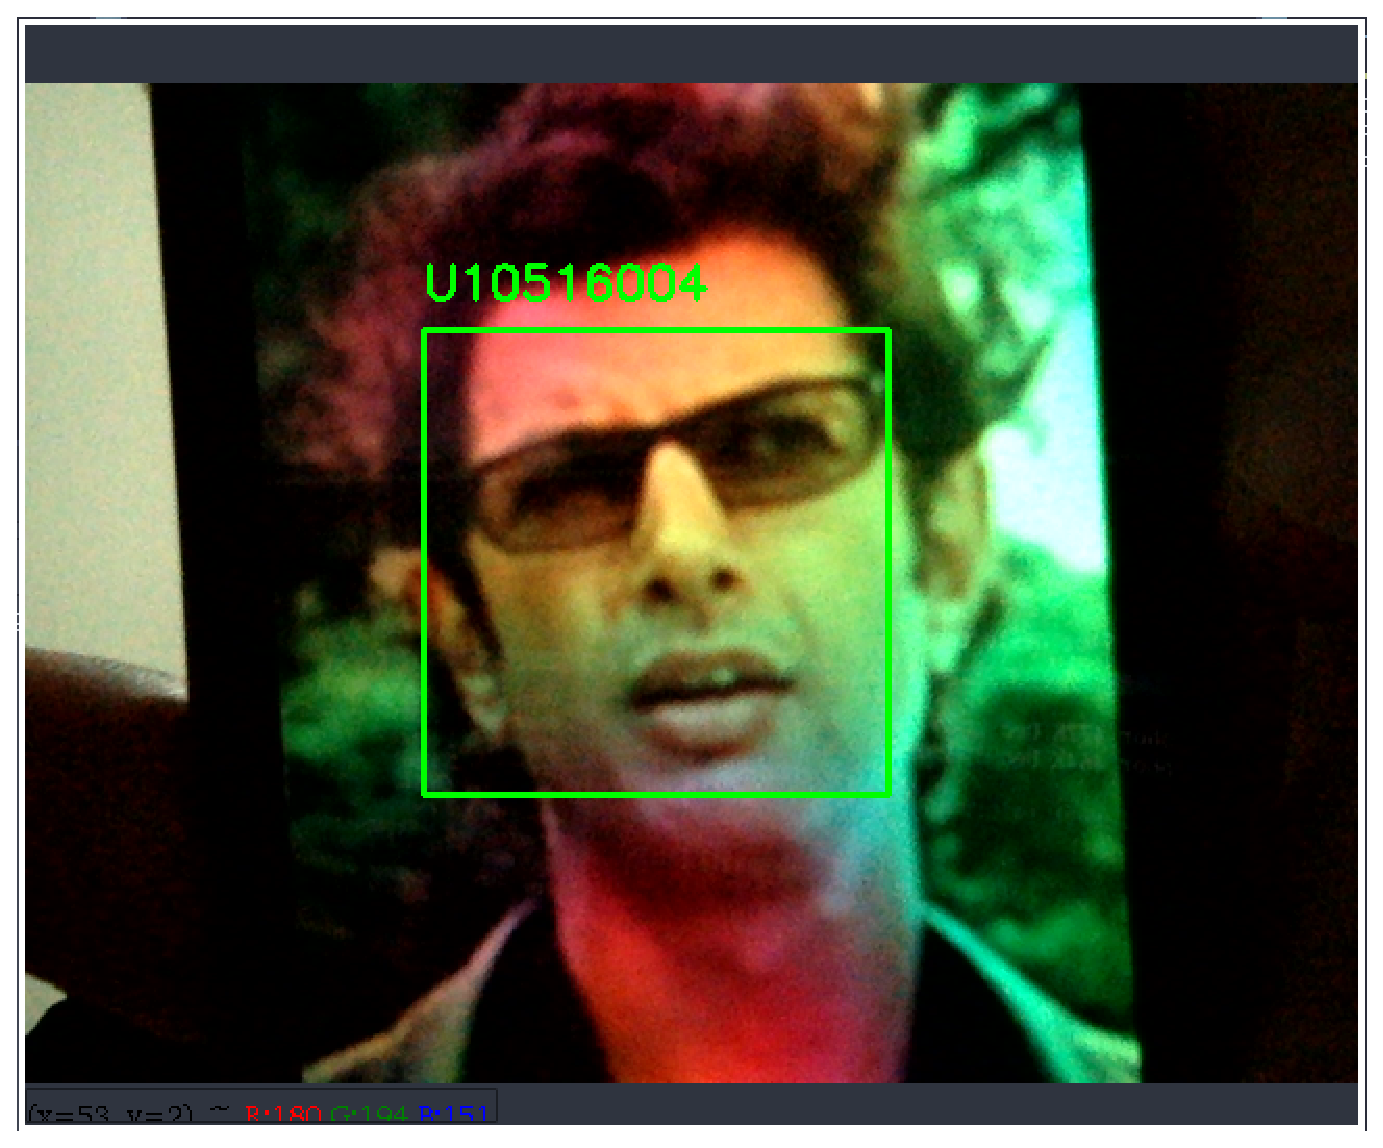
\includegraphics[width=\linewidth]{figures/exp04.eps}
    \caption{U10516004 Ian Malcolm.}
  \end{subfigure}
  \begin{subfigure}[b]{0.32\linewidth}
    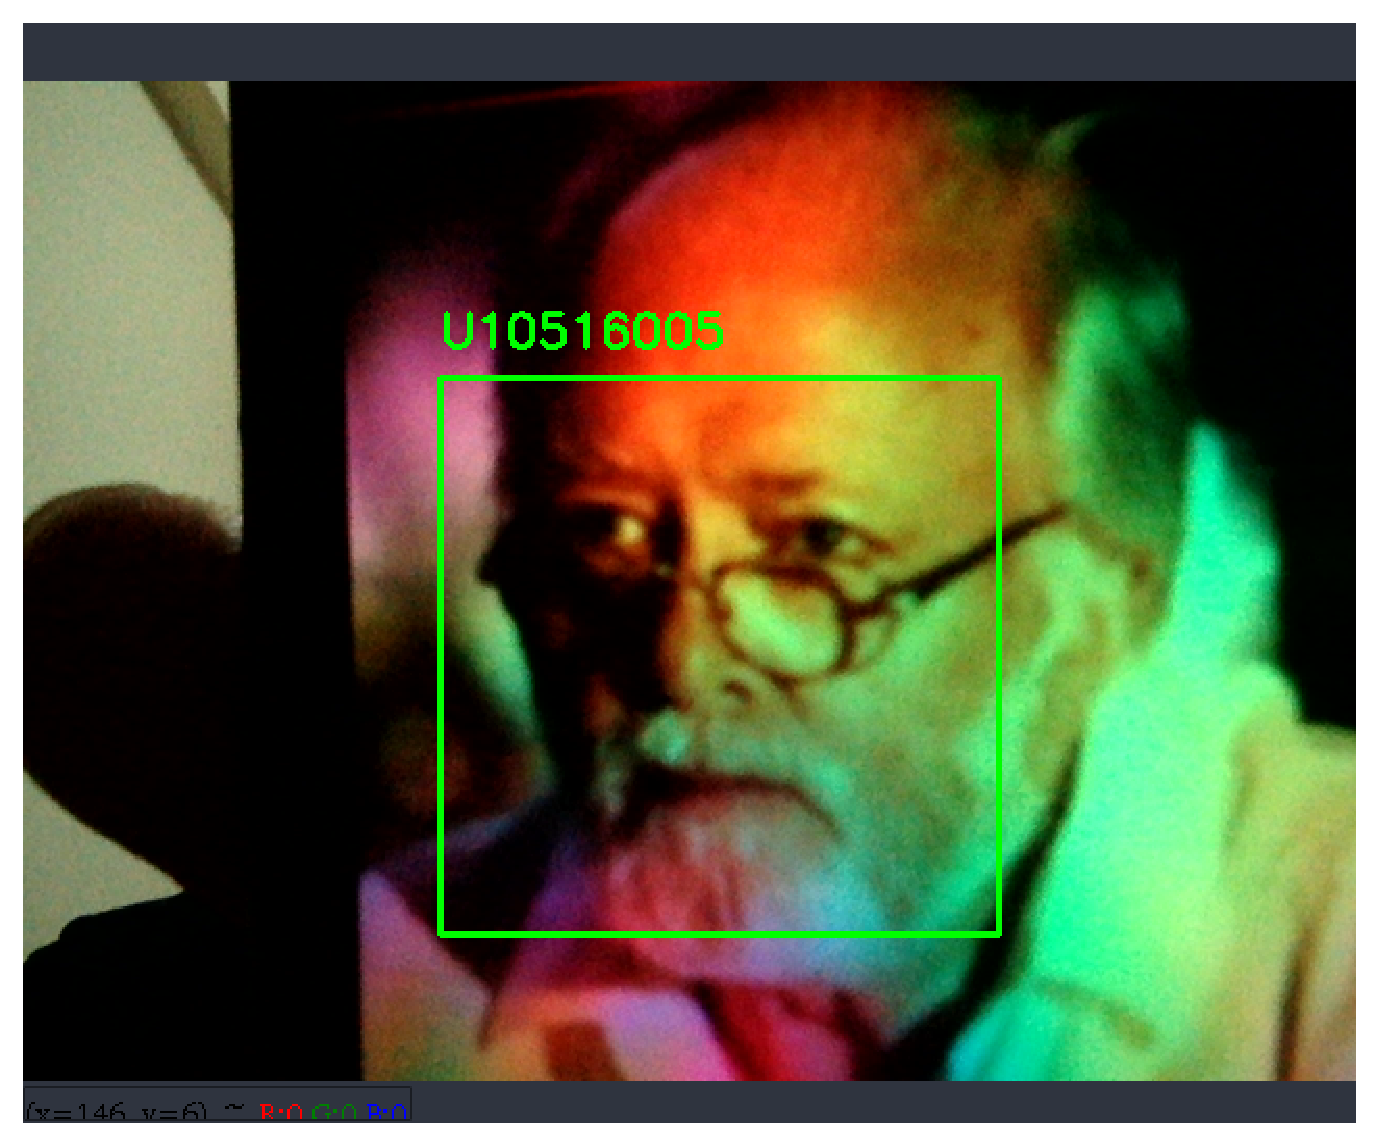
\includegraphics[width=\linewidth]{figures/exp05.eps}
    \caption{U10516005 John Hammond.}
  \end{subfigure}
  \begin{subfigure}[b]{0.32\linewidth}
    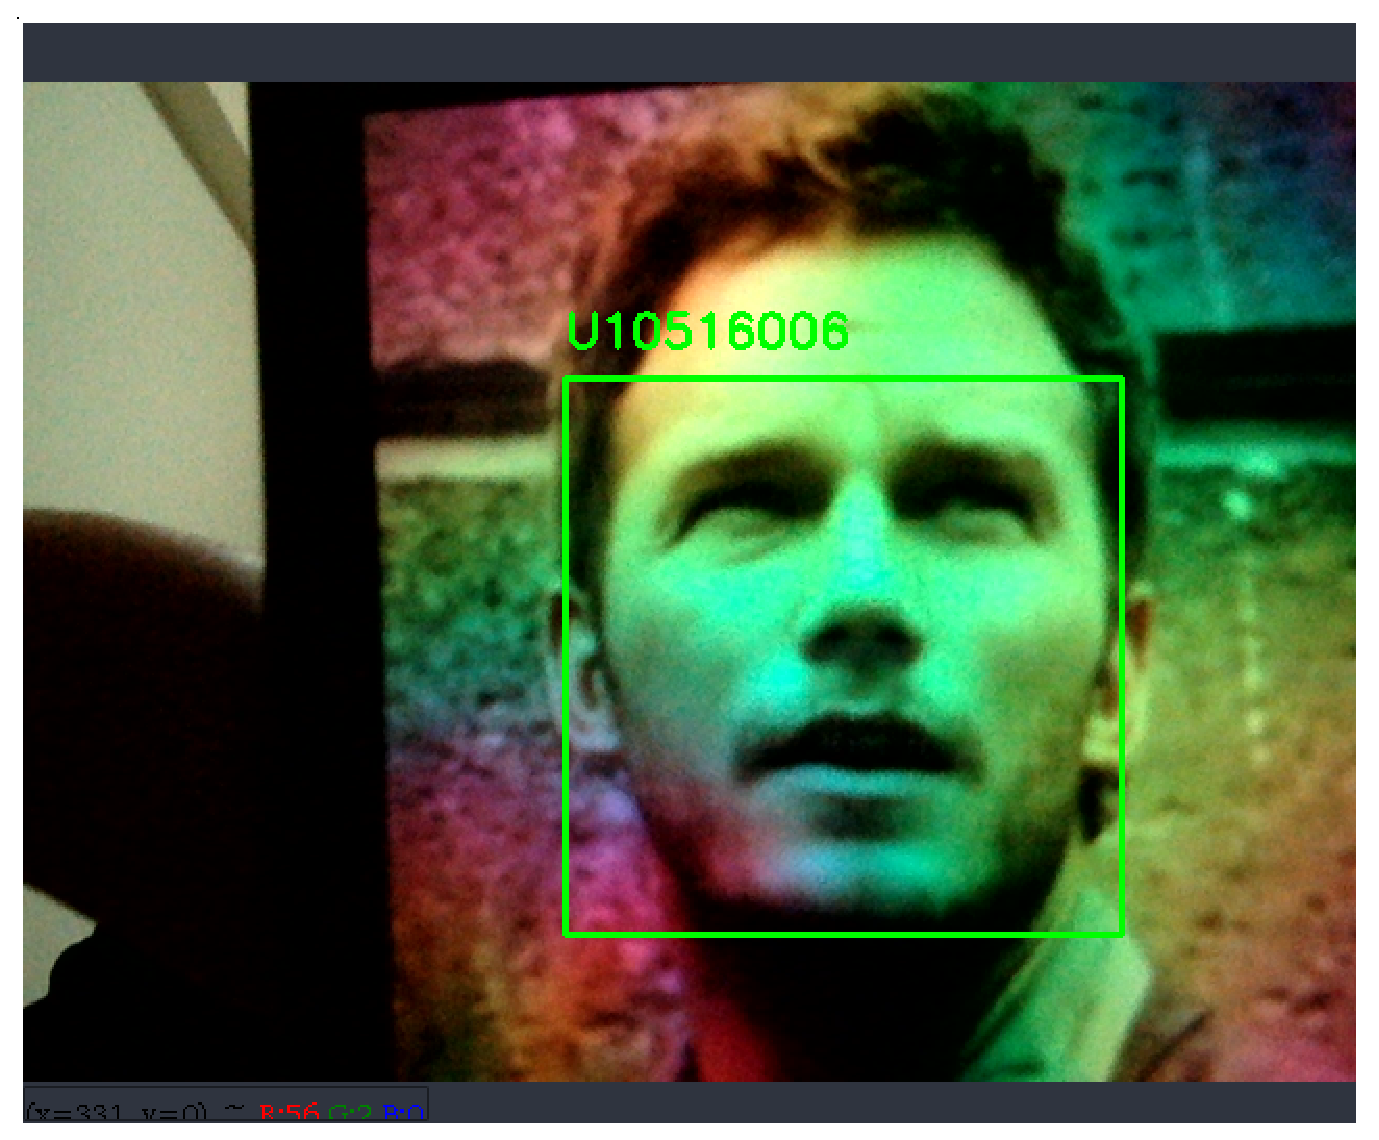
\includegraphics[width=\linewidth]{figures/exp06.eps}
    \caption{U10516006 Owen Grady.}
  \end{subfigure}
  \begin{subfigure}[b]{0.32\linewidth}
    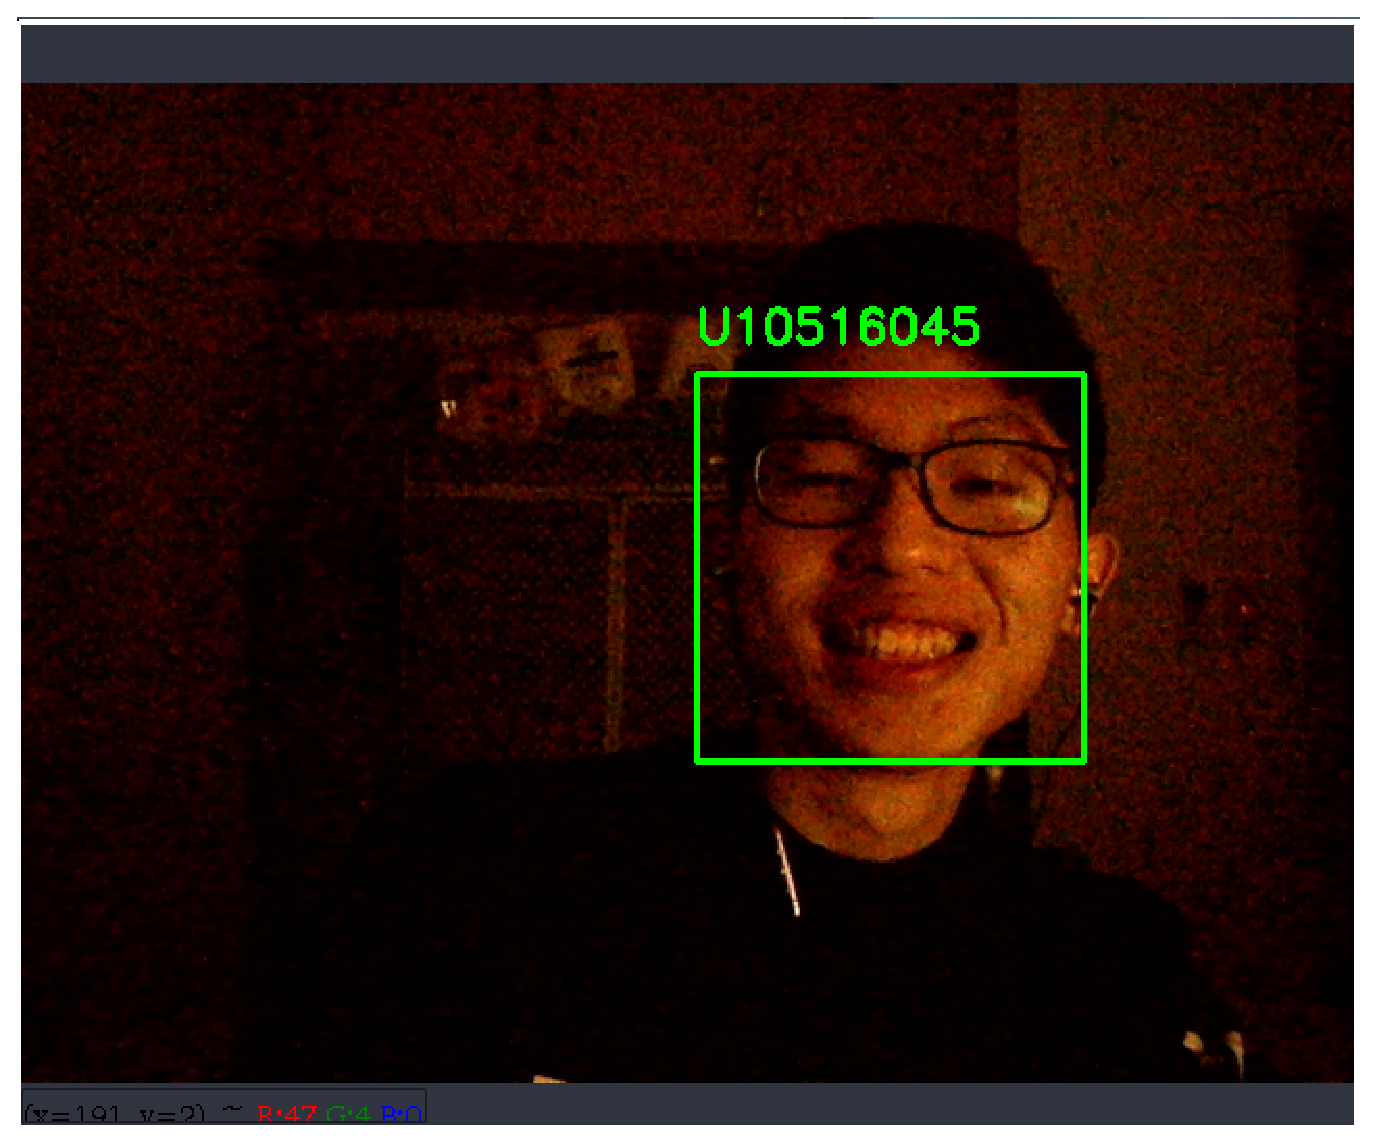
\includegraphics[width=\linewidth]{figures/exp45.eps}
    \caption{U10516045 Guan-Zhong Wang.}
  \end{subfigure}
  \caption{Experimental Result.}
  \label{fig:coffee}
\end{figure}
